\documentclass[tikz,crop=false]{standalone}
\usepackage[paperwidth=297mm,paperheight=216mm,margin=10mm]{geometry} % H4 landscape
\usepackage{tikz}
\usetikzlibrary{arrows.meta,positioning,fit,shapes.multipart,calc,backgrounds,matrix}

% ---- Layering: background < main < foreground ----
\pgfdeclarelayer{bg}
\pgfdeclarelayer{fg}
\pgfsetlayers{bg,main,fg}

\begin{document}
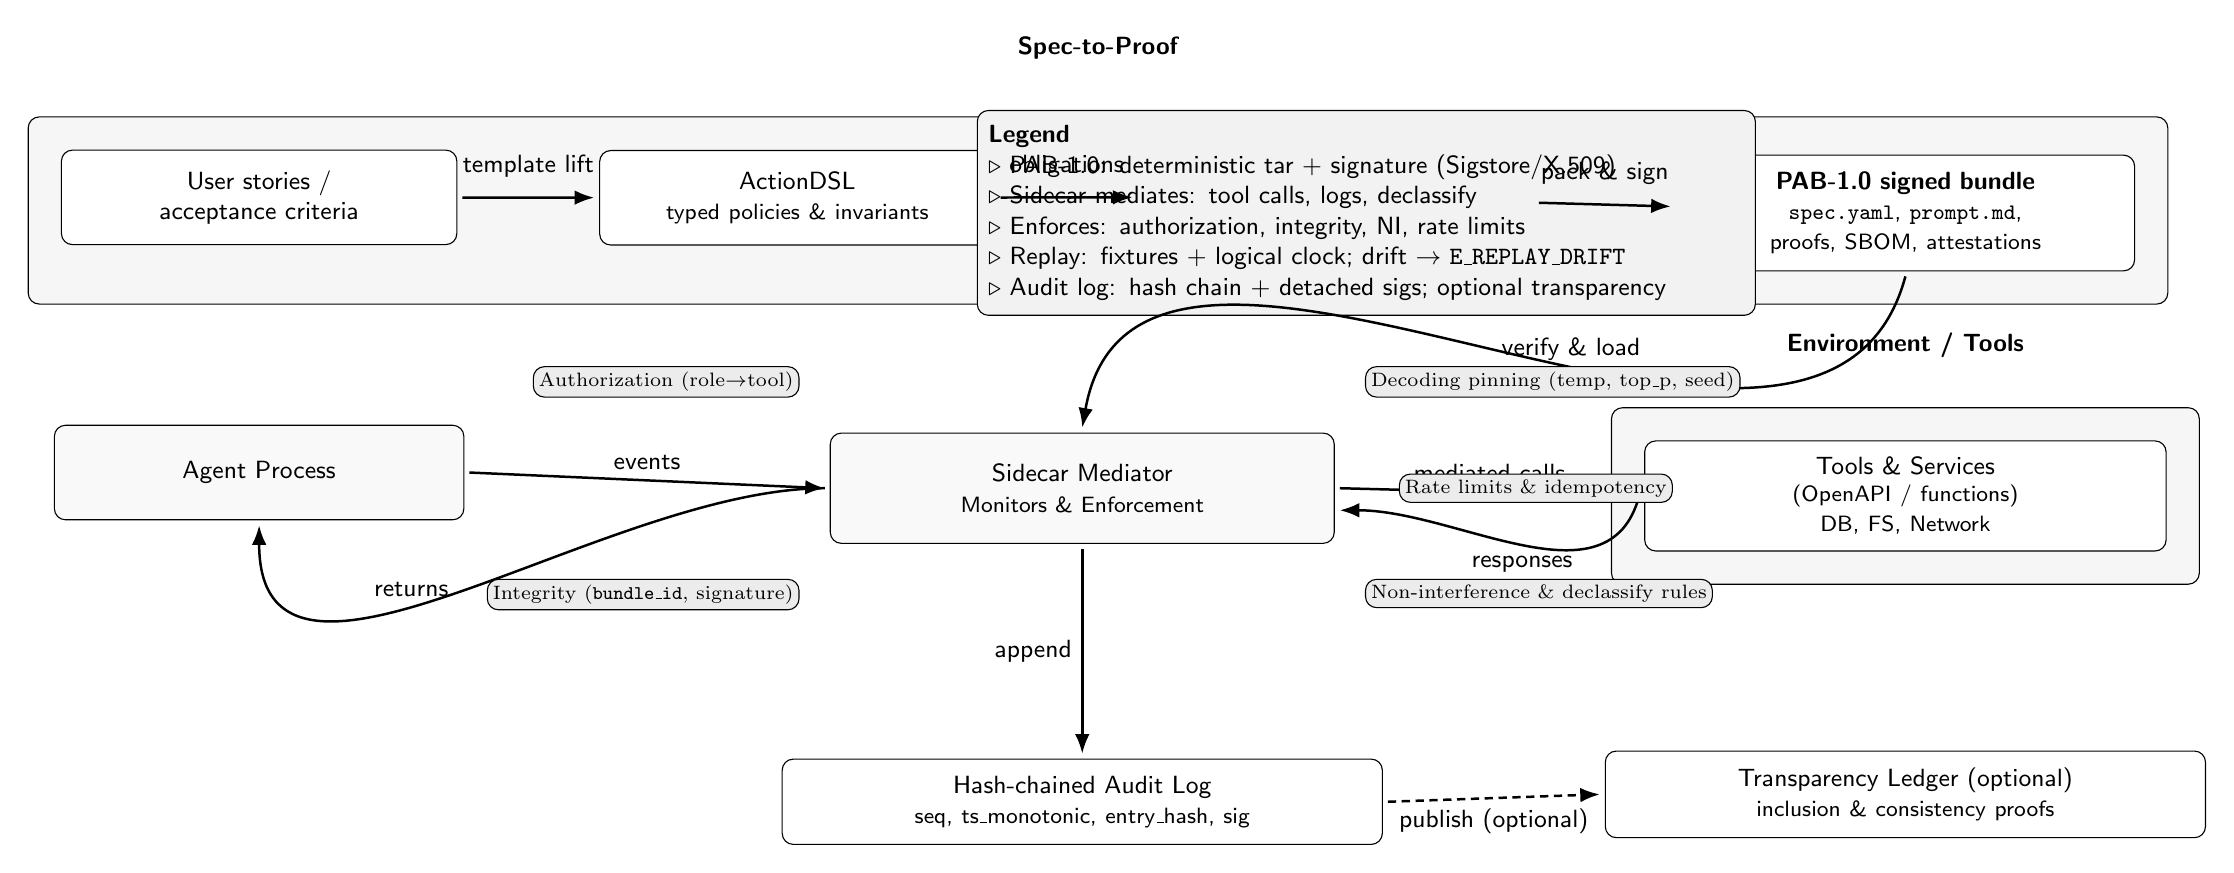
\begin{tikzpicture}[
  remember picture, % allow anchoring to current page
  font=\sffamily\small,
  >=Latex,
  box/.style   ={draw,rounded corners,inner sep=6pt,outer sep=2pt,align=center,fill=white},
  grp/.style   ={draw,rounded corners,inner sep=10pt,outer sep=6pt,align=left,fill=gray!7},
  note/.style  ={draw,rounded corners,inner sep=4pt,fill=gray!10,align=left},
  callout/.style={draw,rounded corners,inner sep=2pt,fill=gray!15,font=\scriptsize},
  arrow/.style ={->,line width=0.9pt},
  dashedarrow/.style={->,densely dashed,line width=0.9pt}
]

% ==================================================
% TOP ROW (matrix = stable spacing, no drift)
% ==================================================
\matrix (toprow) [matrix of nodes,
  nodes={box, minimum height=12mm},
  column sep=18mm, row sep=0mm,
  nodes in empty cells,
] {
  |[name=stories,   text width=46mm]| {User stories /\\ acceptance criteria} &
  |[name=actiondsl, text width=46mm]| {ActionDSL\\ \footnotesize typed policies \& invariants} &
  |[name=lean,      text width=46mm]| {Lean proofs\\ \footnotesize \texttt{BundleSafe}, NI} &
  |[name=pab,       text width=54mm]| {\textbf{PAB-1.0 signed bundle}\\ \footnotesize \texttt{spec.yaml}, \texttt{prompt.md}, proofs, SBOM, attestations} \\
};

% Group frame behind top row
\begin{pgfonlayer}{bg}
  \node[grp, fit=(stories)(pab), label={[yshift=4mm]\bfseries Spec-to-Proof}] (specgrp) {};
\end{pgfonlayer}

% Mid anchor of top row (for vertical alignment)
\node (specmid) at ($(stories)!0.5!(pab)$) {};

% Column anchors to align middle/bottom
\node (col1) at (stories)   {};
\node (col2) at (actiondsl) {};
\node (col3) at (lean)      {};
\node (col4) at (pab)       {};

% ==================================================
% MIDDLE ROW (aligned under columns; generous spacing)
% ==================================================
\node[box, fill=gray!5, minimum width=64mm, minimum height=14mm, below=27mm of specmid] (sidecar)
  {Sidecar Mediator\\ \footnotesize Monitors \& Enforcement};

\node[box, fill=gray!5, minimum width=52mm, minimum height=12mm, below=27mm of col1] (agent)
  {Agent Process};

\node[box, text width=62mm, below=27mm of col4] (tools)
  {Tools \& Services\\ \footnotesize (OpenAPI / functions)\\ DB, FS, Network};

% Group frame behind tools
\begin{pgfonlayer}{bg}
  \node[grp, fit=(tools), label={[yshift=3mm]\bfseries Environment / Tools}] (envgrp) {};
\end{pgfonlayer}

% ==================================================
% BOTTOM ROW (legend left; audit center; ledger right)
% ==================================================
% Reserve vertical space so these sit comfortably above page bottom/legend
\node[box, below=26mm of sidecar, text width=72mm] (audit)
  {Hash-chained Audit Log\\ \footnotesize seq, ts\_monotonic, entry\_hash, sig};

\node[box, below=24mm of tools, text width=72mm] (ledger)
  {Transparency Ledger (optional)\\ \footnotesize inclusion \& consistency proofs};

% ==================================================
% FOREGROUND: connectors + callouts
% ==================================================
\begin{pgfonlayer}{fg}
  % Top row edges (lift labels to clear group title)
  \draw[arrow] (stories)   -- node[above, yshift=1.2mm]{template lift} (actiondsl);
  \draw[arrow] (actiondsl) -- node[above, yshift=1.2mm]{obligations} (lean);
  \draw[arrow] (lean)      -- node[above, yshift=1.2mm]{pack \& sign} (pab);

  % PAB -> Sidecar (curved to avoid group title)
  \draw[arrow] (pab.south) to[out=-105,in=80] node[right, xshift=1mm]{verify \& load} (sidecar.north);

  % Agent <-> Sidecar
  \draw[arrow] (agent.east) -- node[above]{events} (sidecar.west);
  \draw[arrow] (sidecar.west) to[out=180,in=270] node[left]{returns} (agent.south);

  % Sidecar <-> Tools
  \draw[arrow] (sidecar.east) -- node[above]{mediated calls} (tools.west);
  \draw[arrow] (tools.west) to[out=255,in=0] node[below]{responses} ($(sidecar.east)+(0,-0.28)$);

  % Audit path
  \draw[arrow] (sidecar.south) -- node[left]{append} (audit.north);
  \draw[dashedarrow] (audit.east) -- node[below]{publish (optional)} (ledger.west);

  % Callouts — nudged to avoid edges
  \node[callout, above left=3.8mm and 3.2mm of sidecar.north west] {Authorization (role$\rightarrow$tool)};
  \node[callout, above right=3.8mm and 3.2mm of sidecar.north east] {Decoding pinning (temp, top\_p, seed)};
  \node[callout, below left=3.8mm and 3.2mm of sidecar.south west] {Integrity (\texttt{bundle\_id}, signature)};
  \node[callout, below right=3.8mm and 3.2mm of sidecar.south east] {Non-interference \& declassify rules};
  \node[callout, right=7.5mm of sidecar.east] {Rate limits \& idempotency};
\end{pgfonlayer}

% ==================================================
% LEGEND — pinned to bottom-left of the page, above margin, sized to never hit audit
% ==================================================
\node[overlay, remember picture, % overlay so it's anchored to the page, not diagram
      note, align=left, anchor=south west, text width=96mm]
  at ([xshift=10mm,yshift=12mm]current page.south west) { % inside margins
\begin{tabular}{@{}l@{}}
\textbf{Legend}\\
\(\triangleright\) PAB-1.0: deterministic tar + signature (Sigstore/X.509)\\
\(\triangleright\) Sidecar mediates: tool calls, logs, declassify\\
\(\triangleright\) Enforces: authorization, integrity, NI, rate limits\\
\(\triangleright\) Replay: fixtures + logical clock; drift $\to$ \texttt{E\_REPLAY\_DRIFT}\\
\(\triangleright\) Audit log: hash chain + detached sigs; optional transparency
\end{tabular}
};

\end{tikzpicture}
\end{document}
